\documentclass[11pt,a4paper]{article} 
\usepackage[portuges]{babel}
\usepackage[utf8]{inputenc}
\usepackage{graphicx}
\usepackage{listings}
\usepackage{amsthm}
\usepackage{booktabs}
\usepackage{amsfonts}
\usepackage{subcaption}
\usepackage[table,xcdraw]{xcolor}
\graphicspath{{..//images//}}

\title{Física Geral - Relatório de prática - Pêndulo simples}
\author{Juliana Cavalcanti Correa}
\date{Dezembro 2015}


\begin{document}
   
  \maketitle

  \section{Introdução}
  \label{sec:intro}
    
    \paragraph{}
    Nesta prática, o objetivo é obter uma aproximação do valor local da aceleração da gravidade, g, e de sua incerteza $\sigma_g$ a partir de uma série de medidas do período de um pêndulo simples.

    \paragraph{}
    O pêndulo utilizado foi montado de acordo com a Figura \ref{fig:pendulo}, permitindo que uma massa metálica oscilasse livremente em um plano paralelo a uma mesa, presa por uma linha de massa desprezível a uma haste de ferro montada sobre essa mesa.
    
    \paragraph{}
    A aceleração pode ser derivada do período do pêndulo partindo-se do princípio de conservação de energia, que diz que a diferença de energia potencial no ponto mais alto da trajetória (A) e no ponto mais baixo (B) deve ser igual à diferença de energia cinética nos dois pontos, assumindo que a perda de energia pela resistência do ar e outros fatores é pequena o suficiente para ser desprezada, o que é aproximadamente verdade para ângulos pequenos de oscliação..

  \section{Procedimento experimental}

    \paragraph{}
    O primeiro passo do experimento foi conferir os valores esperados das resistências através do código de cores apresentados nos resistores. Os dois utilizados tinham o mesmo código (marrom/preto/laranja/dourado), indicando resistência nominal de $10k\Omega\pm 5\%$.
    \paragraph{}
    Visando garantir o bom funcionamento dos resistores e verificar se eram compatíveis com o valor indicado no código de cores, foi realizada uma etapa preliminar, onde foram tomadas medidas diretas da resistência usando um multímetro analógico e um digital. Com cada um dos dois instrumentos, foram tomadas dez medidas de cada arranjo - cada um dos resistores individualmente e as combinações em série e paralelo descritas na Seção ~\ref{sec:esquema}. O objetivo era garantir que os resistores estavam operando normalmente, sem variações, o que de fato foi constatado: para todos os casos, as dez medições foram iguais. Esses valores estão resumidos na Tabela ~\ref{tab:diretas}.

    \begin{table}[htb!]
      \centering 
      \begin{tabular}{c|cccc}
        \toprule
                               &  R1            &  R2             & série          & paralelo      \\
        \midrule
        cód cores (k$\Omega$)  & $10,0 \pm 0,5 $  & $10,0 \pm 0,5$  & $20,0 \pm 0,7$   & $5,0 \pm 0,3$   \\   
        digital   (k$\Omega$)  & $9,90 \pm 0,17$ & $9,86 \pm 0,17$ & $19,76 \pm 0,29$ & $4,94 \pm 0,11$ \\
        analógico (k$\Omega$)  & $8,0 \pm 0,3$    & $8,0 \pm 0,3$    & $17,8 \pm 0,7$   & $4,5 \pm 0,2$   \\
        \bottomrule
      \end{tabular}
      \caption{Valores das resistências indicados pelo código de cores e medidos com os multímetros digital e analógico, incluindo seus respectivos erros.}
      \label{tab:diretas}
    \end{table}
    
    \paragraph{}
    Para calcular o erro das medidas, também descrito na Tabela ~\ref{tab:diretas}, deveríamos combinar o erro estatístico com o erro do instrumento. Entretanto, como todas as medidas de cada conjunto foram idênticas, não há erro estatístico e, dessa forma, o erro de cada medida é a pŕopria incerteza do instrumento. Segundo os manuais dos fabricantes, essa incerteza no multímetro analógico vale 4\% e no digital 1,2\%+5d, o que equivale a 0,012*R + 0,05, onde R é a resistência medida, visto que as medidas foram tomadas em uma escala com duas casas decimais de precisão.
    \paragraph{}
    Além disso, a incerteza do código de cores dos resistores individuais, indicada pela linha dourada do próprio código, é de $0,5k\Omega$, e o das combinações é derivado a partir desse da seguinte forma:
      \begin{itemize}
        \item Resistores em série (k$\Omega$) = $\sqrt{0,5^{2} + 0,5^{2}}$
        \item Resistores em paralelo (k$\Omega$) = $5^{2}\cdot(\frac{0,5}{10^{2}}+ \frac{0,5}{10^{2}})$
      \end{itemize} 
      
    \paragraph{}
    Em seguida, foram montados os esquemas mostrados na Figura ~\ref{fig:esquemas} usando os mesmos resistores, que haviam sido identificados e numerados na etapa anterior. Foram aplicados, então, dez valores de tensão variando entre 2V e 20V e, para cada valor da tensão, efetuadas dez medidas de corrente para cada arranjo. Os resultados estão sumarizados na Tabela ~\ref{tab:indiretas}.
     
      \begin{table}[htb!]
        \centering
        \begin{tabular}{c|cccc}
         \toprule
                & \multicolumn{4}{c}{i(mA)}        \\
          V (V) & R$_1$   & R$_2$   & R$_{serie}$  & R$_{paralelo}$ \\
          \midrule
          2     & 0.214   & 0.209   & 0.105        & 0.41            \\
          4     & 0.414   & 0.413   & 0.208        & 0.84            \\
          6     & 0.617   & 0.61    & 0.308        & 1.23            \\
          8     & 0.828   & 0.818   & 0.415        & 1.65            \\
          10    & 1.033   & 1.018   & 0.514        & 2.06            \\
          12    & 1.236   & 1.222   & 0.618        & 2.48            \\
          14    & 1.445   & 1.429   & 0.722        & 2.88            \\
          16    & 1.65    & 1.631   & 0.821        & 3.3             \\
          18    & 1.85    & 1.831   & 0.923        & 3.71            \\
          20    & 2.08    & 2.05    & 1.03         & 4.12            \\
          \bottomrule
        \end{tabular}
        \caption{Medidas de corrente para os dois resistores e para os arranjos em série e em paralelo, com valores de tensão variando de 2 a 20V}
        \label{tab:indiretas}
      \end{table}

  \pagebreak
  \section{Tratamento de dados}

    \subsection{Ajuste linear}
      \paragraph{}
      Para verificar a validade da Lei de Ohm, realizamos um ajuste linear utilizando o método dos mínimos quadrados. Esse método busca ajustar uma reta no gráfico V x i, de tal forma a minimizar a soma dos quadrados dos resíduos, que seria dada pela expressão $$\sum\limits_{k=1}^{10}[V_k - (a \cdot i_k + b)]^2$$ Se a relação expressa pela Lei de Ohm for válida, o coeficiente angular \textbf{a} deve ser compatível tanto com as medidas diretas das resistências quanto com os valores indicados nos códigos de cores de R, enquanto o valor do coeficiente linear \textbf{b} deve ser compatível com 0.
      \paragraph{}
      Na Tabela ~\ref{tab:mmq} são descritos os coeficientes angular e linear encontrados com suas incertezas.
     
      \begin{table}[htb!]
        \centering
        \begin{tabular}{c|c|c|c|c}
          \toprule
          arranjo        & R$_1$   & R$_2$   & R$_{serie}$  & R$_{paralelo}$ \\
          \midrule
          a (= $R_{eq}$) & $ 9.69 \pm 0.03$ & $ 9.81 \pm 0.02$  & $ 19.5 \pm 0.04$  & $ 4.86 \pm 0.01$  \\
          b              & $-0.01 \pm 0.04$ & $-0.02 \pm 0.03$  & $-0.05 \pm 0.02$  & $-0.02 \pm 0.02$  \\
          \bottomrule
        \end{tabular}
        \caption{Coeficientes do ajuste linear das medidas de V X i para cada resistor e para os arranjos em série e em paralelo}
        \label{tab:mmq}
      \end{table} 
      
      \paragraph{}
      Os gráficos de V x i dos quatro arranjos podem ser vistos nas Figuras ~\ref{fig:i1} a ~\ref{fig:ip}. As retas descritas pelo ajuste linear são representadas pelas linhas de cor laranja em cada gráfico. Visualmente, é possível perceber que as retas se aproximam dos pontos, indicando que há um comportamento linear, porém, para comprovar, devemos verificar a compatibilidade dos valores medidos para os coeficientes das retas.
  
      \begin{figure}[htb!]
        \centering
        \captionsetup{justification=centering}  
        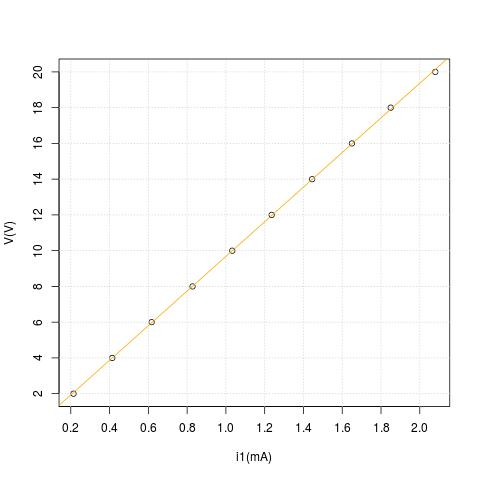
\includegraphics[scale=0.55]{Vi1}
        \caption{Gráfico V x i do resistor 1}
        \label{fig:i1}
      \end{figure}
      
      \begin{figure}[htb!]
        \centering
        \captionsetup{justification=centering}  
        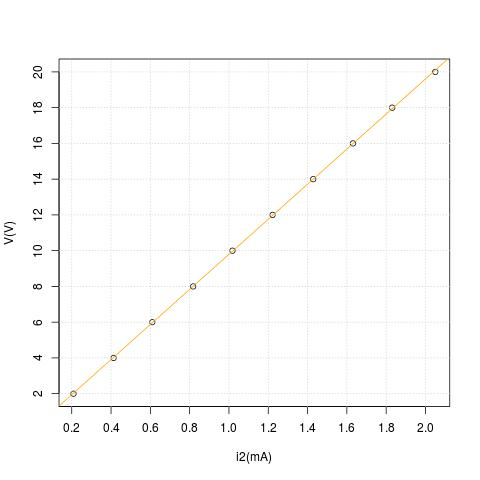
\includegraphics[scale=0.55]{Vi2}
        \caption{Gráfico V x i do resistor 2}
        \label{fig:i2}
      \end{figure}
      
      \begin{figure}[htb!]
        \centering
        \captionsetup{justification=centering}  
        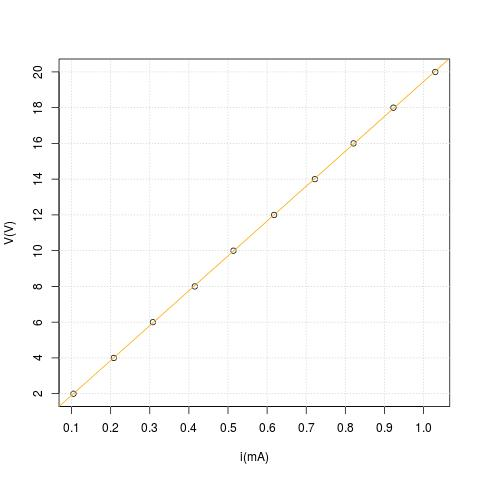
\includegraphics[scale=0.55]{Vis}
        \caption{Gráfico V x i do arranjo de resistores em série}
        \label{fig:is}
      \end{figure}
      
      \begin{figure}[htb!]
        \centering
        \captionsetup{justification=centering}  
        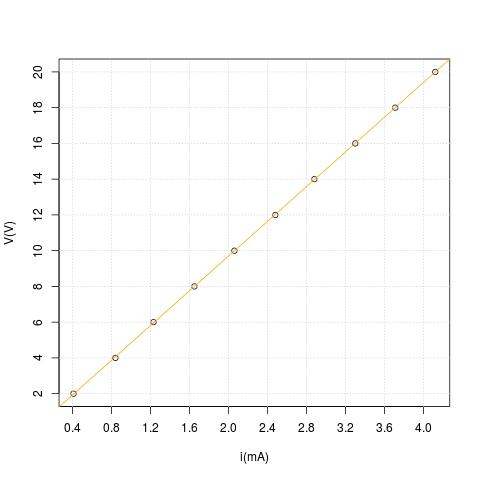
\includegraphics[scale=0.55]{Vip}
        \caption{Gráfico V x i do arranjo de resistores em paralelo}
        \label{fig:ip}
      \end{figure}
      
    \clearpage
    \subsection{Verificação de compatibilidade}
    
      \paragraph{}
      Em primeiro lugar, tentamos verificar a compatibilidade das medidas diretas das resistências obtidas na etapa preliminar com os multímetros analógico e digital, entre si e também com os valores de resistência indicados pelo código de cores.  Para isso, entre cada par de medidas, foram calculadas a discrepância ( $|\bar{x_1}-\bar{x_2}|$ ) e o erro ($\sigma = \sqrt{\sigma_{\bar{x}_1}^2 + \sigma_{\bar{x}_2}^2}$). As medidas são consideradas compatíveis quando a discrepância for menor que 2 vezes o erro. As Tabelas ~\ref{tab:compatccdig}, ~\ref{tab:compatccanalog} e ~\ref{tab:compatdiganalog} resumem os valores.
      \paragraph{}
      Para a comparação da medida do multímetro digital com o valor do código de cores, todos os arranjos têm discrepância menor que $1\sigma$, sendo, portanto, compatíveis. No entanto, a discrepância das medidas do multímetro analógico em relação aos valores do código de cores é maior que $3\sigma$ para os resistores individuais, indicando que a medida é incompatível, e fica entre $2\sigma$ e $3\sigma$ para o arranjo em série, que tem incerteza maior, indicando resultado inconclusivo. O mesmo ocorre na comparação dos dois multímetros - as medidas são incompatíveis para os resistores individuais e inconclusivas para o arranjo em série. Tais discrepâncias podem ser justificadas pela possibilidade da bateria do multímetro analógico estar fraca, resultando em valores sistematicamente menores.

       \begin{table}[htb!]
        \centering
        \begin{tabular}{llll}
        \toprule
                   & Discrepância      & Erro & Compatível                          \\
          \midrule
          R1       & 0.10              & 0.53 & {\color[HTML]{009901} Sim}          \\
          R2       & 0.14              & 0.53 & {\color[HTML]{009901} Sim}          \\
          série    & 0.24              & 0.76 & {\color[HTML]{009901} Sim}          \\
          paralelo & 0.06              & 0.32 & {\color[HTML]{009901} Sim}          \\
          \bottomrule
          
          \end{tabular}
        \caption{Avaliação de compatibilidade entre os valores de resistência indicados pelo código de cores e os medidos com o multímetro digital.}
        \label{tab:compatccdig}
        \end{table}
        
        
       \begin{table}[htb!]
        \centering
        \begin{tabular}{llll}
        \toprule
                   & Discrepância      & Erro & Compatível                          \\
          \midrule
          R1       & 2.00              & 0.59 & {\color[HTML]{CB0000} Não}          \\
          R2       & 2.00              & 0.59 & {\color[HTML]{CB0000} Não}          \\
          série    & 2.20              & 0.99 & {\color[HTML]{646809} Inconclusivo} \\
          paralelo & 0.10              & 0.36 & {\color[HTML]{CB0000} Não}          \\
          \bottomrule
          
          \end{tabular}
        \caption{Avaliação de compatibilidade entre os valores de resistência indicados pelo código de cores e os medidos com o multímetro analógico.}
        \label{tab:compatccanalog}
        \end{table}
        
               \begin{table}[htb!]
        \centering
        \begin{tabular}{llll}
        \toprule
                   & Discrepância      & Erro & Compatível                          \\
          \midrule
          R1       & 1.90              & 0.36 & {\color[HTML]{CB0000} Não}          \\
          R2       & 1.86              & 0.36 & {\color[HTML]{CB0000} Não}          \\
          série    & 1.96              & 0.76 & {\color[HTML]{646809} Inconclusivo} \\
          paralelo & 0.04              & 0.23 & {\color[HTML]{009901} Sim}          \\ 
          \bottomrule
          
          \end{tabular}
        \caption{Avaliação de compatibilidade entre os valores de resistência medidos com os multímetros analógico e digital analógico.}
        \label{tab:compatdiganalog}
        \end{table}
        
      \paragraph{}
      Para finalizar o experimento, buscamos verificar a compatibilidade dos coeficientes obtidos no ajuste linear de V x i com os valores obtidos na etapa preliminar. Como o multímetro analógico apresentou resultados incompatíveis com o digital e com o código de cores já na etapa anterior, optou-se por testar a compatibilidade apenas com os valores do código de cores e com os medidos pelo multímetro digital. Além disso, também é testada a compatibilidade do coeficiente linear (b) com 0. 
      \paragraph{}
      Os resultados estão dispostos nas Tabelas ~\ref{tab:compatajcc} a ~\ref{tab:compatb}, onde se constata que todos os valores são compatíveis. É possível observar também que, como os erros  $\sigma_{a}$ e $\sigma_{b}$ encontrados no ajuste linear são muito pequenos, as incertezas do instrumento de medida e dos próprios resistores (indicada pelo código de cores) prevalecem no cálculo do erro.

       \begin{table}[htb!]
        \centering
        \begin{tabular}{llll}
        \toprule
                   & Discrepância      & Erro & Compatível                          \\
          \midrule
          R1       & 0.31              & 0.50 & {\color[HTML]{009901} Sim}          \\
          R2       & 0.19              & 0.50 & {\color[HTML]{009901} Sim}          \\
          série    & 0.50              & 0.70 & {\color[HTML]{009901} Sim}          \\
          paralelo & 0.14              & 0.20 & {\color[HTML]{009901} Sim}          \\
          \bottomrule
          
        \end{tabular}
        \caption{Avaliação de compatibilidade entre o coeficiente angular da reta obtida no ajuste e os valores de resistência indicados pelo código de cores.}
        \label{tab:compatajcc}
        \end{table}
        
      \begin{table}[htb!]
        \centering
        \begin{tabular}{llll}
        \toprule
                   & Discrepância      & Erro & Compatível                          \\
          \midrule
          R1       & 0.21              & 0.17 & {\color[HTML]{009901} Sim}          \\
          R2       & 0.05              & 0.17 & {\color[HTML]{009901} Sim}          \\
          série    & 0.26              & 0.29 & {\color[HTML]{009901} Sim}          \\
          paralelo & 0.08              & 0.11 & {\color[HTML]{009901} Sim}          \\ 
          \bottomrule
          
        \end{tabular}
        \caption{Avaliação de compatibilidade entre o coeficiente angular da reta obtida no ajuste e os valores de resistência medidos.}
        \label{tab:compatajdig}
      \end{table}
      
      
      \begin{table}[htb!]
        \centering
        \begin{tabular}{llll}
        \toprule
                   & Discrepância      & Erro & Compatível                          \\
          \midrule
          R1       & 0.01              & 0.04 & {\color[HTML]{009901} Sim}          \\
          R2       & 0.02              & 0.03 & {\color[HTML]{009901} Sim}          \\
          série    & 0.05              & 0.02 & {\color[HTML]{009901} Sim}          \\
          paralelo & 0.02              & 0.02 & {\color[HTML]{009901} Sim}          \\ 
          \bottomrule
        \end{tabular}
        \caption{Avaliação de compatibilidade do coeficiente linear da reta com o valor 0.}
        \label{tab:compatb}
      \end{table}

  \section{Conclusão}
      
     \paragraph{}
    Observando a compatibilidade entre o coeficiente angular e o valor da resistência, tanto indicada pelo código de cores quanto medida diretamente com o multímetro, pode-se concluir que, de fato, há um comportamento linear da tensão com a corrente. Juntando essa conclusão com a compatibilidade com 0 do coeficiente linear, verifica-se que as medidas satisfazem a equação V = R * i, ficando completa a previsão da Lei de Ohm. Dessa maneira, o objetivo do experimento foi atingido com sucesso.
    \paragraph{}
     A principal dificuldade observada durante o experimento foi a incompatibilidade das medidas efetuadas com o multímetro analógico, possivelmente devido à bateria do mesmo. Entretanto, isso não influenciou no resultado final, já que as mesmas medidas foram efetuadas também com o multímetro digital.      
\end{document}